%!TEX root = origin_elements_lecture_notes.tex

\chapter{Stardust}\label{ch:stardust}

Researchers around Ed Anders and Roy Lewis at the University of Chicago were puzzling over isotope anomalies found in meteorites. Some primitive meteorites showed strange isotopic compositions in certain noble gas isotopes that did not fit into the Solar System. Furthermore, these isotopic abundances were weird since they could not easily be explained by any chemical process. The researchers separated the meteorite into individual parts in the hope of isolating the carrier of these anomalies, which they ultimately, discovered: interstellar nanodiamonds \citep{lewis87}. For the curious reader, a detailed review on astrophysics with extraterrestrial material was recently presented by \citet{nittler16}.


\section{The Origin of Stardust}

\begin{figure}[tb]
    \centering
    \includegraphics[width=0.9\textwidth]{graphics/stardust/presolar_grains_origin_1600}
    \caption{Schematic of the origin of stardust grains.}
    \label{fig:stardust:origin_of_stardust_schematic}
\end{figure}
The origin of stardust grains is summarized schematically in Figure~\ref{fig:stardust:origin_of_stardust_schematic}
These grains formed in the death throes of dying stars and got subsequently recycled into the interstellar medium. Some of these particles became part of the molecular cloud from which the Solar System formed. Since they represent samples from before the solar nebula, they are also often referred to as presolar grains. During the formation of the first solids in the Solar System, stardust grains were incorporated into meteorite parent bodies. Some primitive meteorites, see discussion in Chapter~\ref{ch:solar_system_abundances}, have preserved these particles up to today. Stardust grains can thus be found in primitive meteorites and can be separated from them for subsequent studies. The grains are especially variable since they carry the nucleosynthetic fingerprint of their parent star.

Stardust grains are generally discovered due to their extreme isotope anomalies, which are very distinct from the solar composition. While their composition cannot be explained by any processes found in the Solar System, they agree astonishingly well with nucleosynthesis predictions of stars, e.g., \ac{sproc} nucleosynthesis in \ac{agb} stars.


\subsection{Types of Stardust Grains}

The most abundant type of stardust grains are nanodiamonds. True to their name, these particles are only a few nanometers in diameter and thus currently still too small in order to study directly in the laboratory. However, recent advances in mass spectrometry have allowed to directly study at least their carbon isotopic composition on a per-grain basis \citep{heck14}. As proposed before \citep{lewis87}, nanodiamonds carry, e.g., the xenon isotopic anomalies. Measuring the size distribution of nanodiamonds and the amount of anomalous xenon, only one in $10^6$ nanodiamonds is actually expected to carry a single xenon atoms. This further complicates research on these phases.

One of the best studied phases of stardust grains are presolar \ac{sic} grains. These particles can be separated from meteorites and thus studied individually in the laboratory. Since \ac{sic} grains frequently occur in sizes of up to several micrometers, they have also been intensively analyzed in the past. Details on these grains are discussion in Section~\ref{sec:stardust:sic_grains}.

Graphite grains can also be gently separated from meteorites. These grains also show up in large sizes, however, graphite can act like a sponge for other elements and thus, the original stellar signal often shows contamination with solar system material.

Finally, in situ detection techniques have allows the search for other types of stardust grains in sections of meteorites. Depending on the type of meteorite, various concentrations of other stardust grains have been found, e.g., silicates, oxides, etc. These grains are usually sub-micrometer in size and thus difficult to analyze. Since they cannot be easily separated from their host meteorite, analyses are more complicated and time-consuming.




\subsection{Separation of Stardust Grains}

Presolar grains such as nanodiamonds and \ac{sic} grains are separated from meteorites using a suite of crushing, freeze-thaw cycles, and chemical treatments. This methodology has also been appropriately referred to as finding the needle in the haystack by burning down the hay. 

Usually, a few grams of a meteorite are taken and first crushed with a mortar and pestle. This breaks the big grains apart. Subsequently, the powder is submerged in water and several freeze-thaw cycles are used in order to break the dust further down into individual component. Once this additional crushing is finished, the burning of the hay begins. Using various acids, material that makes up all the solar system ``stuff'', e.g., the silicates, organic material, etc., are dissolved. After each acid step, remaining solids are separated from the liquid by centrifugation and the liquid is decanted or pipetted off. Finally, only presolar \ac{sic} grains and the hardiest phases that form in the solar system should be left over, among which are \href{https://en.wikipedia.org/wiki/Spinel}{spinels}. These phases have different densities from the stardust grains and can thus be separated further using heavy liquids. For example, spinel has an average density of 3.64\,g\,cm$^{-3}$,\footnote{\url{http://webmineral.com/data/Spinel.shtml}} while \ac{sic} has an average density of 3.21\,g\,cm$^{-3}$.\footnote{\url{http://webmineral.com/data/Moissanite.shtml}}

During all of these steps, extreme care has to be taken in order to (1) not loose the micrometer-sized \ac{sic} grains and (2) to not contaminate them with solar material. Therefore, only the cleanest possible acids and other chemical are used in these separation procedures. These separation procedures take weeks to months and grains need to be subsequently mounted for further analysis. This is usually done by mounting SiC grains onto ultra-pure gold foil.
\begin{figure}[tb]
    \centering
    \includegraphics[width=0.35\textwidth]{graphics/stardust/standard_mount}
    \caption{A standard for presolar grain analysis mounted in the same way as actual samples would be mounted. Due to the high density of the standard, it can actually be seen in this image as rings.}
    \label{fig:stardust:sample_mount}
\end{figure}
Figure~\ref{fig:stardust:sample_mount} shows an image of a sample mount onto which four different standards were loaded. As for presolar grains, standards are drop deposited onto ultra-clean gold. Here, four distinct rings can be seen. Compared to samples, standards are mounted in a higher density, which makes the material visible.


\subsection{In Situ Analyses}

In comparison to stardust grain separations, in situ searches of meteorite slices can also be performed. Here, researchers usually use ion imaging techniques (see next section) in order to search for isotopically anomalous spots in a given meteorite. For example, a meteorite slice can be imaged to search for anomalies in the oxygen isotopic composition. While all phases from the Solar System generally plot in a very constrained area in terms of isotopic ratios, presolar grains can vary massively from the solar composition. Thus, these grains will stick out in ion images as hot spots.



\section{Measurement Techniques}

Many micro- and nanoscale techniques are required in order to study stardust grains. Here we will focus strictly on state-of-the art analysis of the isotopic composition of presolar grains. Further techniques, e.g., to study the crystal structure, of these grains, can be found in the literature \citep[see, e.g.,][and references therein]{nittler16}.

\subsection{Secondary Electron Microscopy}

In order to locate and identify the stardust grains of interest on a gold mount, \acf{sem} is used to image the mount first. Here, an electron beam is scanned over the surface and the intensity of secondary electrons are measured to reconstruct an image. Any kind of microscopy is limited to how small a feature it can detect by its wavelength. This is also known as the Abbe diffraction limit, which states that
\begin{equation}
    d = \frac{\lambda}{2n\sin(\theta)}.
\end{equation}
Here, $d$ is the minimum resolvable distance, $\lambda$ the wavelength, $n$ the refractive index of the medium, and $\theta$ the half-angle of the spot the beam of light is converting to. Usually, $n\sin(\theta)$ is also called the numerical aperture of a system and, in modern microscopes, can achieve values 1.4-1.6. The wavelength of electrons is a lot shorter than the wavelength of light, thus \acp{sem} can achieve a much higher resolution.
\begin{figure}[tb]
    \centering
    \includegraphics[width=\textwidth]{graphics/stardust/sem_mount-s}
    \caption{Small section of a presolar grain gold mount imaged in an \ac{sem}. Identified \ac{sic} grains are circled in purple.}
    \label{fig:stardust:sem_stardust_mount_map}
\end{figure}
Figure~\ref{fig:stardust:sem_stardust_mount_map} shows a fraction of a stardust gold mount imaged in the \ac{sem}. Here, backscattered electrons, which elastically scatter of the sample, were detected for generating the image. Heavy elements backscatter electrons more strongly than light ones. Therefore, gold is shown as a bright surface while \ac{sic} grains are dark. 

Imaging mounts however is not good enough since separation of stardust grain can always leave some other material behind. Therefore, \ac{sic} also have to be identified by elemental mapping to ensure that silicon and carbon are present. This is usually done by \acf{edx}. Irradiating the sample with the electron beam in an \ac{sem} excites the sample's electrons. When these electrons fall back into their ground state they emit X-rays, which are characteristic of the element itself. By analyzing these X-rays, the composition of the imaged sample can be determined. In Figure~\ref{fig:stardust:sem_stardust_mount_map}, identified \ac{sic} grains are marked with purple circles. Imaging and mapping of stardust grain mounts can generally be done automatically and can take up to sever days, depending on the resolution required. These maps usually contain thousands of images, poorly overlapping image boarders can be seen in Figure~\ref{fig:stardust:sem_stardust_mount_map}. Subsequent marking of the grain mount can also be automated, e.g., using imaging software such as ImageJ.\footnote{\url{https://imagej.nih.gov/ij/}}


\subsection{Mass Spectrometry}

While elemental analysis that rely on electron transitions can be done in a non-destructive way, no method to date exists to analyze the overall isotopic composition. However, mass spectrometry techniques with high enough spatial resolution in order to analyze individual grains have been developed. Here, two of these techniques that are regularly applied to stardust analysis are described in detail. These two techniques are the main drivers to analyze the stardust grains for their isotopic nucleosynthesis fingerprints.

The principal setup of every mass spectrometer can be broken into three main parts. First, an ion source must be present that can take the given sample and ionize its constituents. In the case of presolar grains the ion source needs to remove material from the grain and ionize it. Second, a mass analyzer then separates the ions by their respective mass-over-charge ($m/q$) ratio. Third, these separated ions must be detected in a detector system.


\paragraph{NanoSIMS} The \acf{nanosims} instrument is built by the French company CAMECA.\footnote{\url{https://www.cameca.com/}} It has been available commercially for around 20\,years and, during this time, has been updated several times. 
\begin{figure}[tb]
    \centering
    \includegraphics[width=0.6\textwidth]{graphics/stardust/nanosims}
    \caption{Schematic inner working of a \ac{nanosims}. Credit: Eden Camp via \href{https://en.wikipedia.org/wiki/Nanoscale_secondary_ion_mass_spectrometry}{Wikipedia}.}
    \label{fig:stardust_nanosims_schematic}
\end{figure}
Figure~\ref{fig:stardust_nanosims_schematic} shows a schematic of the inner workings of a \ac{nanosims}. 
In a NanoSIMS, sample material is removed from the surface using an ion gun, usually either by using Cs$^{+}$ or O$^{-}$ ions. Depending on the exact setup, the ion beams can be focused down to usually tens of nanometers. The size of this ion beam also defines the spatial resolution that can be achieved by the instrument. When the ion beam hits the surface, sample material is sputtered off. Some small fraction of this sample material is ionized directly due to the interaction with the ion beam. This directly ionized fraction, which is usually $\ll1\%$ of the total sputtered material, is then focused with various electrostatic lenses and transported to a magnetic sector. When passing through the magnetic field $\vec{B}$, the Lorentz force $\vec{F}_L$ will separate the ions by $m/q$:
\begin{equation}
    \vec{F}_L = q(\vec{E} + \vec{v} \times \vec{B})
\end{equation}
The electric field $\vec{E}$ can be neglected in a magnetic sector and the separation is solely due to the magnetic field $\vec{B}$. Individual, separated ion beams are then detected. Depending on the amount of signal, this detection either takes place via secondary electron detectors, which amplify the signal and are thus used for low count rates, or using Faraday cups that simple measure the total number of ions arriving using a current meter.

In order to calibrate the detector and the ionization probability, standards with known composition are often used. For example: when measuring presolar \ac{sic} grains for their carbon and silicon isotopic composition, terrestrial \ac{sic} can be used as a standard material. Since stardust grains show large isotopic variations compared to material that originated from within the Solar System, these standard materials can be assumed to have solar composition.

While \ac{nanosims} is a valuable technique to analyze stardust grains, the low secondary ion yield achieved by sputtering limits the technique's applicability to major elements in these samples. Furthermore, since ions are separated by $m/q$, isobaric interferences can occur depending on the elements of interest. For example, when analyzing the iron isotopic composition of a given stardust grain, the abundance of \ex{58}Fe cannot be measured since it would be overshadowed by \ex{58}Ni (see, e.g., Figure~\ref{fig:s-process:feni_chartnuc}). Similarly, \ex{64}Ni cannot be distinguished from \ex{64}Zn. Other techniques are thus required in order to remove isobaric interferences and achieve higher sensitivity. 


\paragraph{RIMS}

To achieve higher sensitivity and suppress isobaric interferences, \acf{rims} can be used to analyze stardust grains. 
\begin{figure}[tb]
    \centering
    \includegraphics[width=0.7\textwidth]{graphics/stardust/rims_schematic}
    \caption{The inner workings of \ac{rims}. Details are described in the text.}
    \label{fig:stardust:rims_schematic}
\end{figure}
Figure~\ref{fig:stardust:rims_schematic} shows a schematic of the inner workings of a \ac{rims} instrument. Numbered steps in the figure are also numbered in the following text. Sample material from a target are removed (1) either using an ion gun, similar to \ac{nanosims}, or a desorption laser. For stardust grain analysis, sample material is generally removed using a desorption laser, which can achieve a spatial resolution of down to $\sim1\,\mu$m. After sample removal, a cloud of neutral atoms (2) and secondary ions exists above the sample. Secondary ions are then ejected from the system by pulsing the extractor optics to high voltages, thus removing these ions from the cloud. Neutral atoms, left behind after this ejection, are then ionized resonantly (3) using tunable \acf{tisa} lasers. The ions are then extracted into a \acf{tof} mass spectrometer, the mass analyzer. Finally, the total flight time of the ions is detected and recorded. This procedure is repeated in modern RIMS instruments at frequencies of 1\,kHz and above. Thus, over time an overall mass spectrum of the sample and its isotopic composition is acquired.

Resonance ionization is highly mass selective. 
\begin{figure}[tb]
    \centering
    \includegraphics[width=0.49\textwidth]{graphics/stardust/fe_ionization_scheme}
    \includegraphics[width=0.49\textwidth]{graphics/stardust/ni_ionization_scheme}
    \caption{Resonance ionization schemes for iron (left) and nickel (right). Figures were created using a \ac{rims} scheme drawer available on \href{https://github.com/RIMS-Code/RIMSSchemeDrawer}{GitHub}.}
    \label{fig:stardust:fe_ni_ionization_schemes}
\end{figure}
Figure~\ref{fig:stardust:fe_ni_ionization_schemes} shows two resonance ionization schemes for iron (left) and nickel (right). Each scheme uses multiple steps in order to ionize an element of interest. These individual steps are highly element specific, which therefore mostly eliminates isobaric interferences in \ac{rims}. Furthermore, since ionization works on the neutral atoms, which are by far the majority of the sputtered or desorbed material from the sample, \ac{rims} is also much more sensitive than, e.g., \ac{nanosims}. \citet{savina18} have shown an overall useful yield for uranium measurements of 38\%. This means that 38\% of all atoms removed from a specific sample have been detected afterwards. However, the laser requirements makes \ac{rims} more complicated and to-date, no commercial mass spectrometer is available. In fact, only two \ac{rims} exist worldwide that focus on stardust analysis, namely the \ac{chili} at the University of Chicago and the \ac{lion} instrument at Lawrence Livermore National Laboratory. 

After ionization, isotopes are separated by $m/q$ in the \ac{tof} mass analyzer. Here, the extractor gives each ion the same amount of energy. Depending on the voltage field the ions go through, their energy becomes $E_\mathrm{el} = q U$, where $q$ is their charge and $U$ is the voltage field. This energy is equal to the kinetic energy $E_\mathrm{kin} = 0.5 m v^2$ of the individual ions. Since the ions have different masses, they will end up having different energies and thus different velocities. Heavier isotopes arrive at the detector later and for a given distance $d$, the total flight time is 
\begin{equation}
    t \propto \sqrt{\frac{m}{q}}.
\end{equation}
The proportionality constant depends on the instrumental setup. 

\begin{figure}[tb]
    \centering
    \includegraphics[width=\textwidth]{graphics/stardust/feni_ms}
    \caption{Simultaneous measurement of iron and nickel by \ac{rims}. The top panel shows the overlap of the two spectra at mass 58, in the bottom spectrum these peaks are separted by shifting the timing of the ionization lasers. Figure created with \href{https://veusz.github.io}{Veusz}.}
    \label{fig:stardust:fe_ni_rims_ms}
\end{figure}
Figure~\ref{fig:stardust:fe_ni_rims_ms} shows a \ac{rims} measurement of all iron and nickel isotopes using the ionization schemes shown in Figure~\ref{fig:stardust:fe_ni_ionization_schemes}. Simultaneous analysis of these two elements show the isobaric inferences at mass 58 (see top panel). With \ac{rims} however, the ionization is not dependent on the ion sputtering event, but rather on the laser ionization pulses. Since \ac{tof} mass spectrometry requires the whole system to be pulses, ionization timings can simply be moved with respect to each other in order to shift mass peaks apart. For the bottom panel in Figure~\ref{fig:stardust:fe_ni_ionization_schemes} this has been done for the iron and nickel measurements. The nickel ionization lasers fire around 200\,ns after the iron ionization lasers, which results in an apparent mass shift. Thus, all isotopes can be detected without isobaric interferences. 

\begin{figure}[tb]
    \centering
    \includegraphics[width=\textwidth]{graphics/stardust/lion}
    \caption{The \ac{lion} instrument at Lawrence Livermore National Laboratory.}
    \label{fig:stardust:lion_photo}
\end{figure}
While many more pages could be written on the beauty of \ac{rims} and its advantages, the curious reader shall hereby be referred to a recently published book chapter \citep{savina21}. An open-access \ac{pdfdoc} version can also be found on the U.S. Department of Energy's Office of Science and Technology Website.\footnote{\url{https://www.osti.gov/servlets/purl/1763939}} Finally, Figure~\ref{fig:stardust:lion_photo} shows an image of the \ac{lion} instrument at Lawrence Livermore National Laboratory. Six tunable \ac{tisa} lasers are shown on the left, the mass spectrometer stands on the right-hand side of the image. The reflectron is out of view on top of the photograph.




\section{Silicon Carbide Grains} \label{sec:stardust:sic_grains}

After having extensively discussed the separation and measurement techniques to analyze stardust grains, let us in brief see what measurements of these grains show. The discussion here mainly focuses on presolar grain classification. More analysis and comparisons with \ac{sproc} models will be discussed in the reading.


\subsection{Notation}

Stardust grains are generally analyzed by mass spectrometry for their isotopic composition. While elemental concentrations can be measured as well, such analyses are preferentially used to trace stardust grain condensation processes and not necessarily nucleosynthesis itself. Isotope measurements are usually expressed as ratios with respect to the most abundant isotope. While direct ratios are used for huge differences, smaller anomalies are usually expressed a permil deviations from the solar composition as so-called $\delta$-values. For any given isotope ratio $^{i}X/^{j}X$ of element $X$ can be written in $\delta$-notation as:
\begin{equation}
    \delta\left(\frac{^iX}{^jX}\right) = \delta {^{i}}X_{j} =  \left[\frac{\left(\frac{^iX}{^jX}\right)_\mathrm{sample}}{\left(\frac{^iX}{^jX}\right)_\odot} - 1\right] \times 1000 \qquad (\permil) \label{eqn:stardust:delta_notation}
\end{equation}
Here, the expression in square brackets defines the $\delta$-value. Multipling this value by 1000 is generally done in order to express this deviation in permil.


\subsection{Classification of \ac{sic} grains}

\begin{figure}[tb]
    \centering
    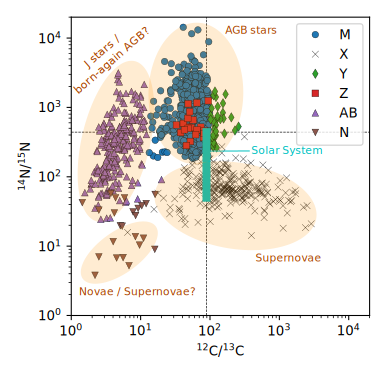
\includegraphics[width=0.49\textwidth]{graphics/stardust/sic_n_c_all}
    \includegraphics[width=0.49\textwidth]{graphics/stardust/sic_si_3iso_all}
    \caption{Nitrogen, carbon, and silicon isotopic composition of analyzed \ac{sic} grains. Data taken from the presolar grain database}
    \label{fig:stardust:classification_c_n_si_data}
\end{figure}
Figure~\ref{fig:stardust:classification_c_n_si_data} shows \ac{sic} the nitrogen isotopic ratio as a function of the carbon isotopic ratio (left) and a silicon three isotope plot (right) for \ac{sic} grain measurements. The axes in the left figure show isotope ratios directly and are both scaled logarithmically. This demonstrates the huge variations in the carbon and nitrogen isotopic composition that stardust grains manifest. Note that the cyan box in the middle shows the total variation, especially of nitrogen isotopes, in the Solar System. Until measurements using samples from the Genesis spacecraft were performed \citep{marty11}, the actual nitrogen isotopic composition of the Sun was poorly understood since large variations of this isotope ratio are found in the Solar System. The range shown in Figure~\ref{fig:stardust:classification_c_n_si_data} (left) is taken from \citet{fueri15}. 

The nitrogen and carbon isotopic compositions can be associated with various nucleosynthetic sources. Clearly established astrophysical sites exist for mainstream (M) and type X presolar grains.\footnote{Type X presolar grains were originally named for their eXtreme isotope ratios.} Type Y and Z grains likely originated from AGB stars as well, probably though from stars with subsolar metallicities. Type AB grains were originally defined as two different groups, however, more data showed one population and these measurements were thus grouped together. Recent studies however indicate multiple origins for type AB grains again. Finally, Type N grains were originally thought to come from novae, however, more studies have shown that surely part of their population originated in supernovae. 

The silicon isotopes, shown on the right in Figure~\ref{fig:stardust:classification_c_n_si_data} as $\delta$-valeus also show a lot of spread. Noticeable features are that X grains seem to be heavily enriched in \ex{28}Si compared to the Solar System. Mainstream grains, originating from AGB stars, all lie on a slope 1.4 line and are for the most part enriched in \ex{29}Si and \ex{30}Si compared to the Solar System.

While measurements of nitrogen, carbon, and silicon are indicative of a stardust grain's origin, other smoking gun measurement have in fact proven the sample's provenance. For grains from supernovae, measurements have shown that they condensed with live \ex{44}Ti, a \ac{slr} with a half-life of $t_{\nicefrac{1}{2}} = 60$\,a. After incorporation, \ex{44}Ti decayed to its stable daughter \ex{44}Ca, which occurs in stardust grains from supernovae in large abundances. Stardust grains from \ac{agb} stars on the other hand show typical \ac{sproc} patterns for elements like strontium, zirconium, molybdenum, etc., thus clearly showing their origin.



\subsection{Constraining \textit{s}-process nucleosynthesis}

\begin{figure}[tb]
    \centering
    \includegraphics[width=0.6\textwidth]{graphics/stardust/zr_s-proc}
    \caption{Zirconium isotope measurements by \citet{barzyk07} in comparison with \ac{agb} star models by \citet{lugaro18}.}
    \label{fig:stardust:zr_comparison_barzyk_lugaro}
\end{figure}
The clear \ac{sproc} signatures in \ac{sic} M grains not only show their provenance, but can also be analyzed in order to better understand the parent stars they formed in.
Figure~\ref{fig:stardust:zr_comparison_barzyk_lugaro} shows zirconium isotope measurements by \citet{barzyk07} in comparison with \ac{agb} star models by \citet{lugaro18}. The $\delta^{96}\mathrm{Zr}_{94}$ ratio shows the amount of branching that takes place in the star, see, e.g., Figures~\ref{fig:s-process:zrmo_chartnuc} and~\ref{fig:s-process:branching_zr95}. If all other parameters are left the same, heavier stars will activate the \ex{22}Ne$(\alpha,n)$ neutron source more efficiently since the temperature at the bottom of the helium intershell is higher. Thus, \ex{95}Zr can be branched more effectively, yielding a higher production of \ex{96}Zr. In Figure~\ref{fig:stardust:zr_comparison_barzyk_lugaro}, all thermal pulses are plotted with symbols and not just lines if the carbon-to-oxygen ratio in the convective envelope exceeds unity. This elemental ratio is required for \ac{sic} to form in the stellar envelope. If more oxygen is present in the envelope, all silicon will form bonds with oxygen assuming a perfectly mixed envelope. Since \ac{sic} can only condense when $\mathrm{C}/\mathrm{O}>1$, the grains can also only trap the nucleosynthetic fingerprint of their parent star at that moment. 

In recent years, significant process has been made on \ac{sproc} nucleosynthesis, especially thanks to efforts by Nan Liu and collaborators. The curious reader is point to check out her publications for further study.\footnote{\url{https://scholar.google.com/citations?user=dGoIdFgAAAAJ}}


\subsection{Supernova condensations}

In addition to studying the \ac{sproc}, \ac{sic} X grains can also be used to analyze output from \acp{sn}. While the measurement techniques are identical to other \ac{sic} grains, the interpretation of the data is more difficult. Studies of \ac{agb} stars have the advantage that everything formed from a homogeneous composition in the convective envelope. \acp{sn} on the other hand are generally only modeled in 1D but clearly show asymmetric explosion patterns in 3D. Inhomogeneous mixing is difficult to constraint.

Recent advances have been made into interpreting \acp{sn} nucleosynthesis and subsequent 3D explosions in the context of stardust analyses \citep{bose21}. These models however still have significant issues and can only constraint some measurements. A comprehensive comparison between 3D \acp{sn} models and stardust data currently remains elusive at best.


\section{Reading}

The reading for this chapter focuses in general on observations that elaborate on stardust. Please read \citet{merrill52}, a fundamental manuscripts that shows that the \ac{sproc} indeed takes place in \ac{agb} stars. In addition, please read \citet{savina04}, a study that first detected the decay products of technetium in \ac{sic} M grains. This work is commonly referred to as the smoking-gun measurement to show that \ac{sic} M grains originated from \ac{agb} stars. The following list of questions might help with your reading:
\begin{itemize}
    \item How and when does \citet{merrill52} mention the discovery of technetium in S-type stars?
    \item Which isotope of technetium did \citet{merrill52} likely observe? Why are the other long-lived isotopes of technetium not produced in the \ac{sproc}?
    \item Can you speculate on how / why Paul Merrill is the sole author of this study?
    \item Which \ac{sproc} signatures have been discovered in stardust prior to the work by \citet{savina04}? Why is the work by \citet{savina04} required to prove that \ac{sic} M grains indeed originated from \ac{agb} stars?
    \item What is the ``standard-size'' \ex{13}C-pocket?
    \item How do \citet{savina04} show that the measured \ex{99}Ru anomaly indeed originates from decay of \ex{99}Tc in the stardust grains?
    \item What are the ``N'' and ``G'' components?
    \item What is meant by the statements in \citet{savina04} that \ex{99}Tc behaves like an \textit{s}-isotope while \ex{99}Ru behaves like an \textit{p}-isotope? Why is this the case?
\end{itemize}
